\documentclass[a4paper,12pt]{article} 
\usepackage[T2A]{fontenc}			
\usepackage[utf8]{inputenc}			
\usepackage[english,russian]{babel}	
\usepackage{amsmath,amsfonts,amssymb,amsthm,mathtools} 
\usepackage[colorlinks, linkcolor = blue]{hyperref}
\usepackage{upgreek}\usepackage[left=2cm,right=2cm,top=2cm,bottom=3cm,bindingoffset=0cm]{geometry}
\usepackage{graphicx}
\usepackage{multirow}
\usepackage{xcolor}
\author{Дорогинин Д.В.}
\title{3.3.3. Опыт Милликена.}
\date{\today}
\begin{document}
\maketitle
\newpage
\textbf{Цель работы}: измерение элементарного заряда методом масляных капель.


\textbf{В работе используются}: плоский конденсатор в защитном кожухе, измерительный микроскоп, электростатический вольтметр, электронный секундомер, переключатель напряжений, пульверизатор с маслом. 
\section*{Теория}
Если элементарный заряд существует, то все заряды будут ему кратны. В опыте будут измерятся заряды капелек масла, несущих несколько элементарных зарядов.\\
Для измерения заряда будем исследовать движение капелек в электрическом поле. Уравнение движения капли при свободном падении
\begin{equation}
m \dfrac{dv}{dt}=mg-F_{\text{тр}},
\end{equation}
где $m$ -- масса капли, $v$ -- её скорость, $F_{\text{тр}}=6\pi \eta rv = kv$ -- сила вязкого трения, $r$ -- радиус капли, $\eta$ -- коэффициент вязкости воздуха. Отсюда получаем 
\begin{equation}
v = \dfrac{mg}{k}\left(1 - e^{-kt/m}\right).
\end{equation}
Скорость установится на
$$
v_{\text{уст}}=\dfrac{mg}{k}=\dfrac{2}{9}\dfrac{\rho}{\eta}gr^2,
$$
где $\rho$ -- плотность масла. Установление этой скорости происходит с постоянной
$$
\tau = \dfrac{m}{k}=\dfrac{2}{9}\dfrac{\rho}{\eta}r^2
$$
Обозначая $h$ путь капли, пройденный за $t_0$, получаем формулу для её радуса:
\begin{equation}
r = \sqrt{\dfrac{9\eta h}{2\rho gt_0}}.
\end{equation}
В случае движения в электрическом поле конденсатора с разностью потенциалов $V$ и расстоянием $l$ между пластинами получаем уравнение движения
\begin{equation}
m \dfrac{dv}{dt}=\dfrac{qV}{l}-mg-kv,
\end{equation}
Новое слагаемое не влияет на $\tau$, новая установившаяся скорость
$$
v_{\text{уст}}'=\dfrac{qV/l - mg}{k}.
$$
Если $t$ -- время подъёма на высоту $h$, то можно получить формулу заряда капли:
$$
\dfrac{qV}{kl}-v_{\text{уст}}=v_{\text{уси}}'=\dfrac{h}{t};
$$
$$
k=6\pi \eta r  = 6\pi \eta  \sqrt{\dfrac{9\eta h}{2\rho gt_0}};
$$
\begin{center}
$\Rightarrow$ \fbox{$q = 9\pi \sqrt{\dfrac{2\eta^3 h^3}{g\rho}}\cdot \dfrac{l(t_0+t)}{Vt^{3/2}_0t}$}
\end{center}
\section*{Описание установки}
\begin{center}
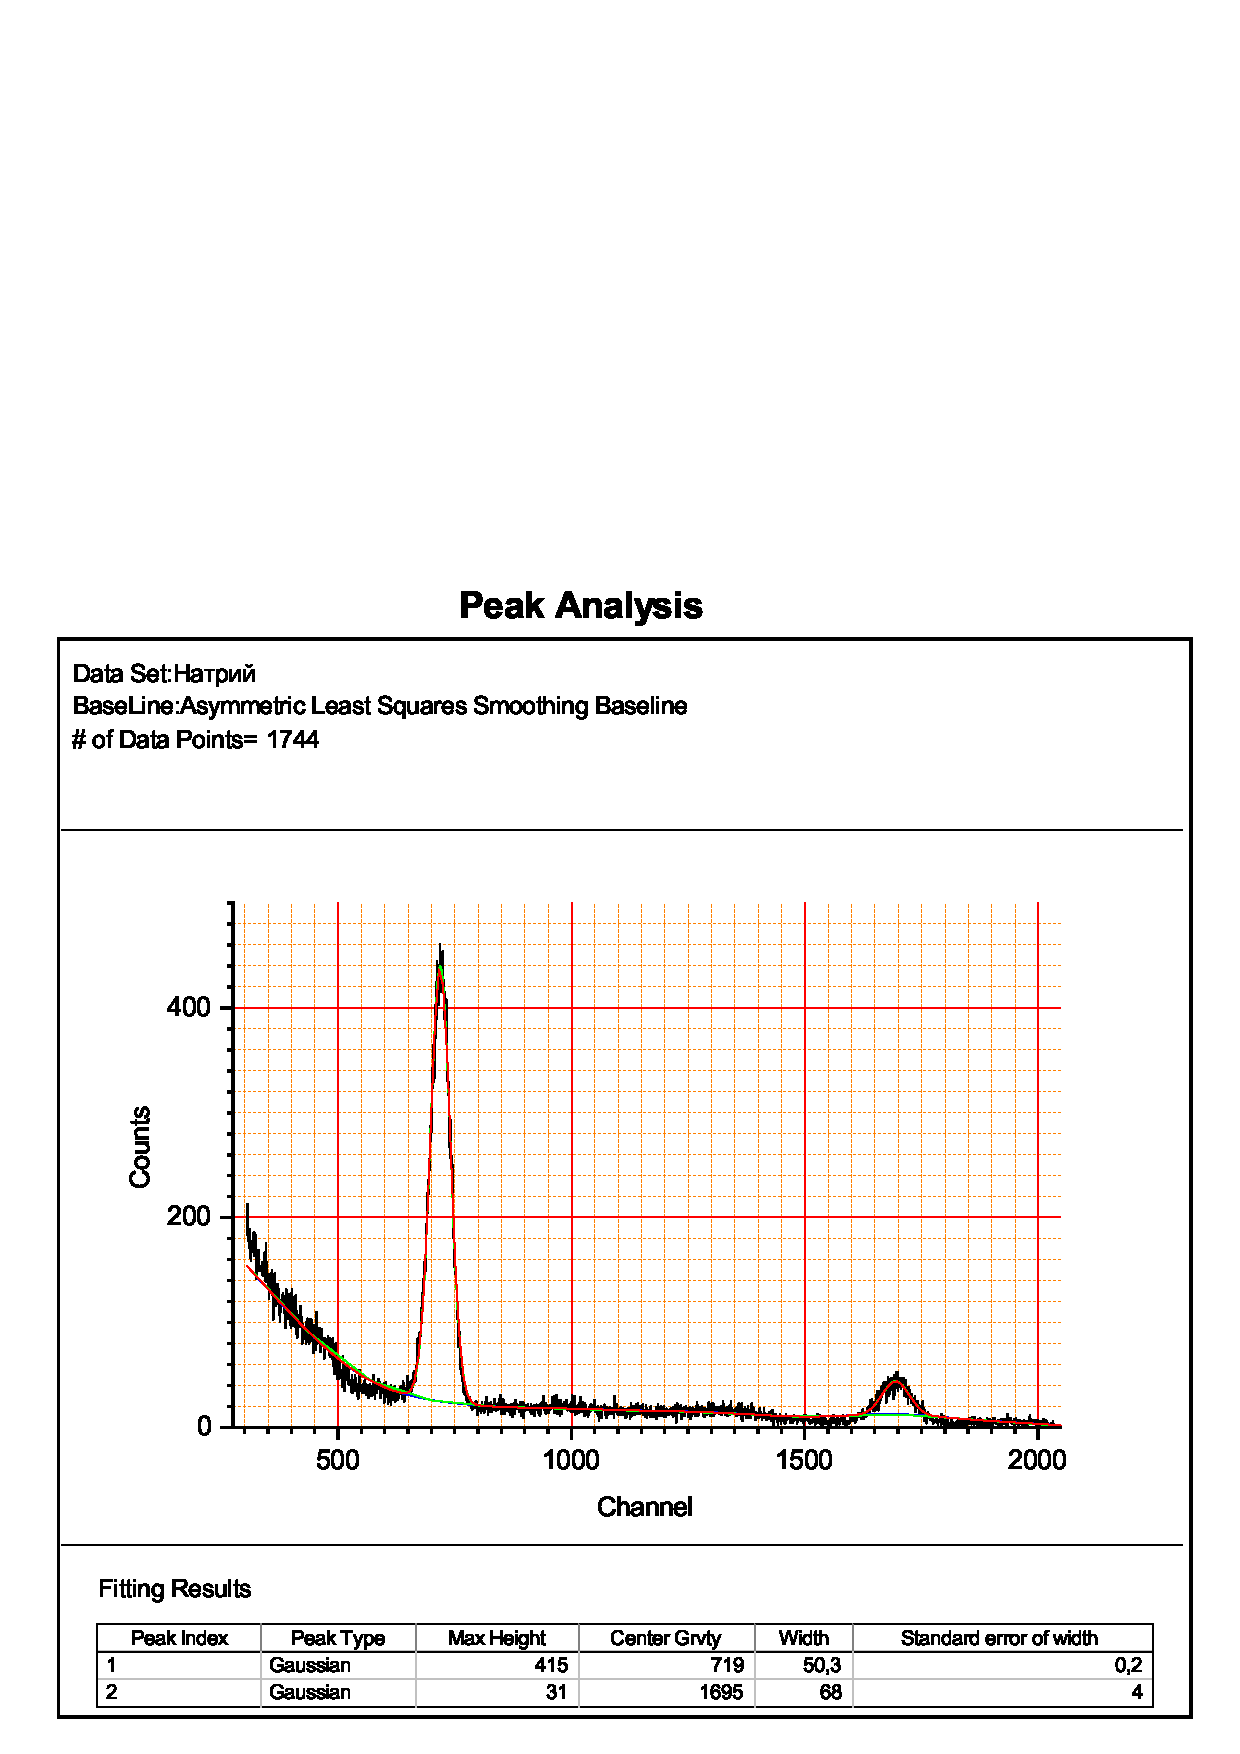
\includegraphics[scale=0.6]{1.png}
\end{center}
Схема преставлена на рисунке. Масло разбрызгивается пульверизатором, попадает на конденсатор $C$ через небольное отверстие, приобретая заряд засчёт трения о воздух.\\
Напряжение подаётся с выпрямителя и измеряется вольтметром $V$. Ключ $K$ позволяет менять направление поля кондексатора. При замыкании конденсатор разряжается в $R \approx 10~\text{МОм}$.\\
Для наблюдения за каплями установлен микроскоп, в фокальной плоскости окуляра которого  виден ряд горизонтальных линий с предварительно определённым расстоянием между ними. Время движения капель замеряется электронным секундомером.
\section*{Ход работы}
\begin{enumerate}
\item Оценим величину напряжения $V$, которое нужно для подъёма капель, несущих от 1 до 5 запрядов электрона на высоту $h = 1~\text{мм}$, задав $t_0 \approx t = 20~\text{с}$:
$$
V =  9\pi \sqrt{\dfrac{(2\eta h/t)^3}{g\rho}}\cdot \dfrac{l}{q} \approx 200 \div 1000~\text{В}.
$$
\item Влючаем осветитель. Не включая поле, слегка надавим на грушу пульверизатора и пронаблюдаем за движением облачка масляных капель.
\item Настроим окуляр на резкое изображение делений. Затем сфокусируем на появившихся каплях.
\item В начале опыта дадим каплям без поля 5-10 секунд свободно падать, чтобы крупные успели упасть на нижнюю пластину.\\
Из оставшихся выберем одну и произведём с ней серию измерений, наблюдая её падение под действием силы тяжести и подъём под действием электрического поля, тем самым измерив $t_0$ и $t$ 5-10 раз. Такие измерения проделаем для 15 капель, каждый раз фиксируя $V$ и имея в виду, что заряд капли может поменятся. В опыте $h = 0.2$ мм.
\newpage
\begin{table}[t]
\centering
\begin{tabular}{|c|c|c|c|c|c|c|c|c|c|c|c|c|c|}
\hline
$U$, В               & 500  & 400   & 400   & 400   & 270    & 270   & 270  & 600   & 400   & 400  & 515   & 515   & 515  \\ \hline
    $h$    & 2    & 1     & 1     & 1     & 1      & 1     & 1    & 1     & 1     & 1    & 1     & 1     & 1    \\ \hline
\multirow{11}{*}{} & 8.7  & 13.82 & 12.25 & 14.35 & 10.96  & 11.4  & 7.57 & 9.9   & 11.28 & 9.57 & 10.12 & 12.7  & 8.75 \\ \cline{2-14} 
                   & 8.3  & 17.84 & 16.97 & 15.72 & 10.87  & 8.88  & 6.91 & 10.65 & 10.25 & 9.82 & 10.47 & 13.18 & 8.42 \\ \cline{2-14} 
                   & 8.05 & 16.7  & 13.92 & 12.32 & 9.82   & 10.25 & 6.9  & 11.58 & 9.67  & 9.53 & 10.45 & 8.53  & 8.46 \\ \cline{2-14} 
                   & 8.5  & 15.99 & 13.9  & 8.91  & 10     & 9.98  & 6.33 & 13.15 & 10.35 & 9.93 & 10.7  & 12.44 & 7.95 \\ \cline{2-14} 
                   & 8.55 & 16.15 & 13.98 & 15.05 & 11.22  & 14.03 & 7.13 & 9.18  & 11.41 & 9.51 & 9.43  & 11.68 & 8.9  \\ \cline{2-14} 
                   & 8.3  & 14.5  &       &       &        & 9.98  &      &       &       &      &       &       &      \\ \cline{2-14} 
                   & 7.95 &       &       &       &        &       &      &       &       &      &       &       &      \\ \cline{2-14} 
                   & 8.26 &       &       &       &        &       &      &       &       &      &       &       &      \\ \cline{2-14} 
                   & 8.33 &       &       &       &        &       &      &       &       &      &       &       &      \\ \cline{2-14} 
                   & 8.25 &       &       &       &        &       &      &       &       &      &       &       &      \\ \cline{2-14} 
                   & 8.22 &       &       &       &        &       &      &       &       &      &       &       &      \\ \hline
$t_0$, с              & 8.31 & 15.83 & 14.20 & 13.27 & 10.57  & 10.75 & 6.97 & 10.89 & 10.59 & 9.67 & 10.23 & 11.71 & 8.50 \\ \hline
2            & 5.5  & 3.01  & 4.18  & 4.4   & 10.14  & 3.41  & 7.25 & 3.5   & 5.45  & 4.53 & 4.31  & 3.43  & 5.25 \\ \hline
\multirow{10}{*}{} & 5.42 & 2.36  & 3.42  & 3.95  & 11.77  & 3.68  & 7.17 & 3.33  & 6     & 4.6  & 4.23  & 3.01  & 5.23 \\ \cline{2-14} 
                   & 5.69 & 2.56  & 3.66  & 4.03  & 13.256 & 3.38  & 7.31 & 3.48  & 5.74  & 3.88 & 4.03  & 3.13  & 5.3  \\ \cline{2-14} 
                   & 5.35 & 2.2   & 3.8   & 3.97  & 10.36  & 2.86  & 7.59 & 3.4   & 5.43  & 4.23 & 4.4   & 2.61  & 4.95 \\ \cline{2-14} 
                   & 5.12 & 2.71  &       & 3.13  & 11.83  & 3.05  & 8.4  & 3.53  & 4.95  & 4.15 & 4.06  &       & 4.91 \\ \cline{2-14} 
                   & 5.52 &       &       & 3.75  &        & 4.1   &      &       &       &      &       &       &      \\ \cline{2-14} 
                   & 5.18 &       &       &       &        &       &      &       &       &      &       &       &      \\ \cline{2-14} 
                   & 5.56 &       &       &       &        &       &      &       &       &      &       &       &      \\ \cline{2-14} 
                   & 5.33 &       &       &       &        &       &      &       &       &      &       &       &      \\ \cline{2-14} 
                   & 5.48 &       &       &       &        &       &      &       &       &      &       &       &      \\ \cline{2-14} 
                   & 5.95 &       &       &       &        &       &      &       &       &      &       &       &      \\ \hline
$t$, с                   & 5.46 & 2.57  & 3.77  & 3.87  & 11.47  & 3.41  & 7.54 & 3.45  & 5.51  & 4.28 & 4.21  & 3.05  & 5.13 \\ \hline
\end{tabular}
\end{table}
\item Для оценки точности <<подвесим>> одну каплю в поле, а затем отключим его и измерим время падения на расстояние 2-3 клеток. Оценим заряд этой капли, полагая $t=\infty$.\\
Полученное среднее время $t_0 = 23.8~\text{с}$ для $U = 180~\text{В}$, капля проходила одно $h$. Тогда 
$$
\delta q =9\pi \sqrt{\dfrac{2\eta^3 h^3}{g\rho}} \lim\limits_{t\rightarrow \infty}  \dfrac{l(t_0+t)}{Vt^{3/2}_0t} = 2 \cdot 10^{-22}~\text{Кл}
$$
Это демонстрирует низкую погрешность метода измерения.
\end{enumerate} 
\section*{Обработка данных}
\begin{enumerate}
\item Для всех капель рассчитаем значения $q$. Нанесём их их на числовую прямую, домножив на $10^{19}$.

\begin{center}
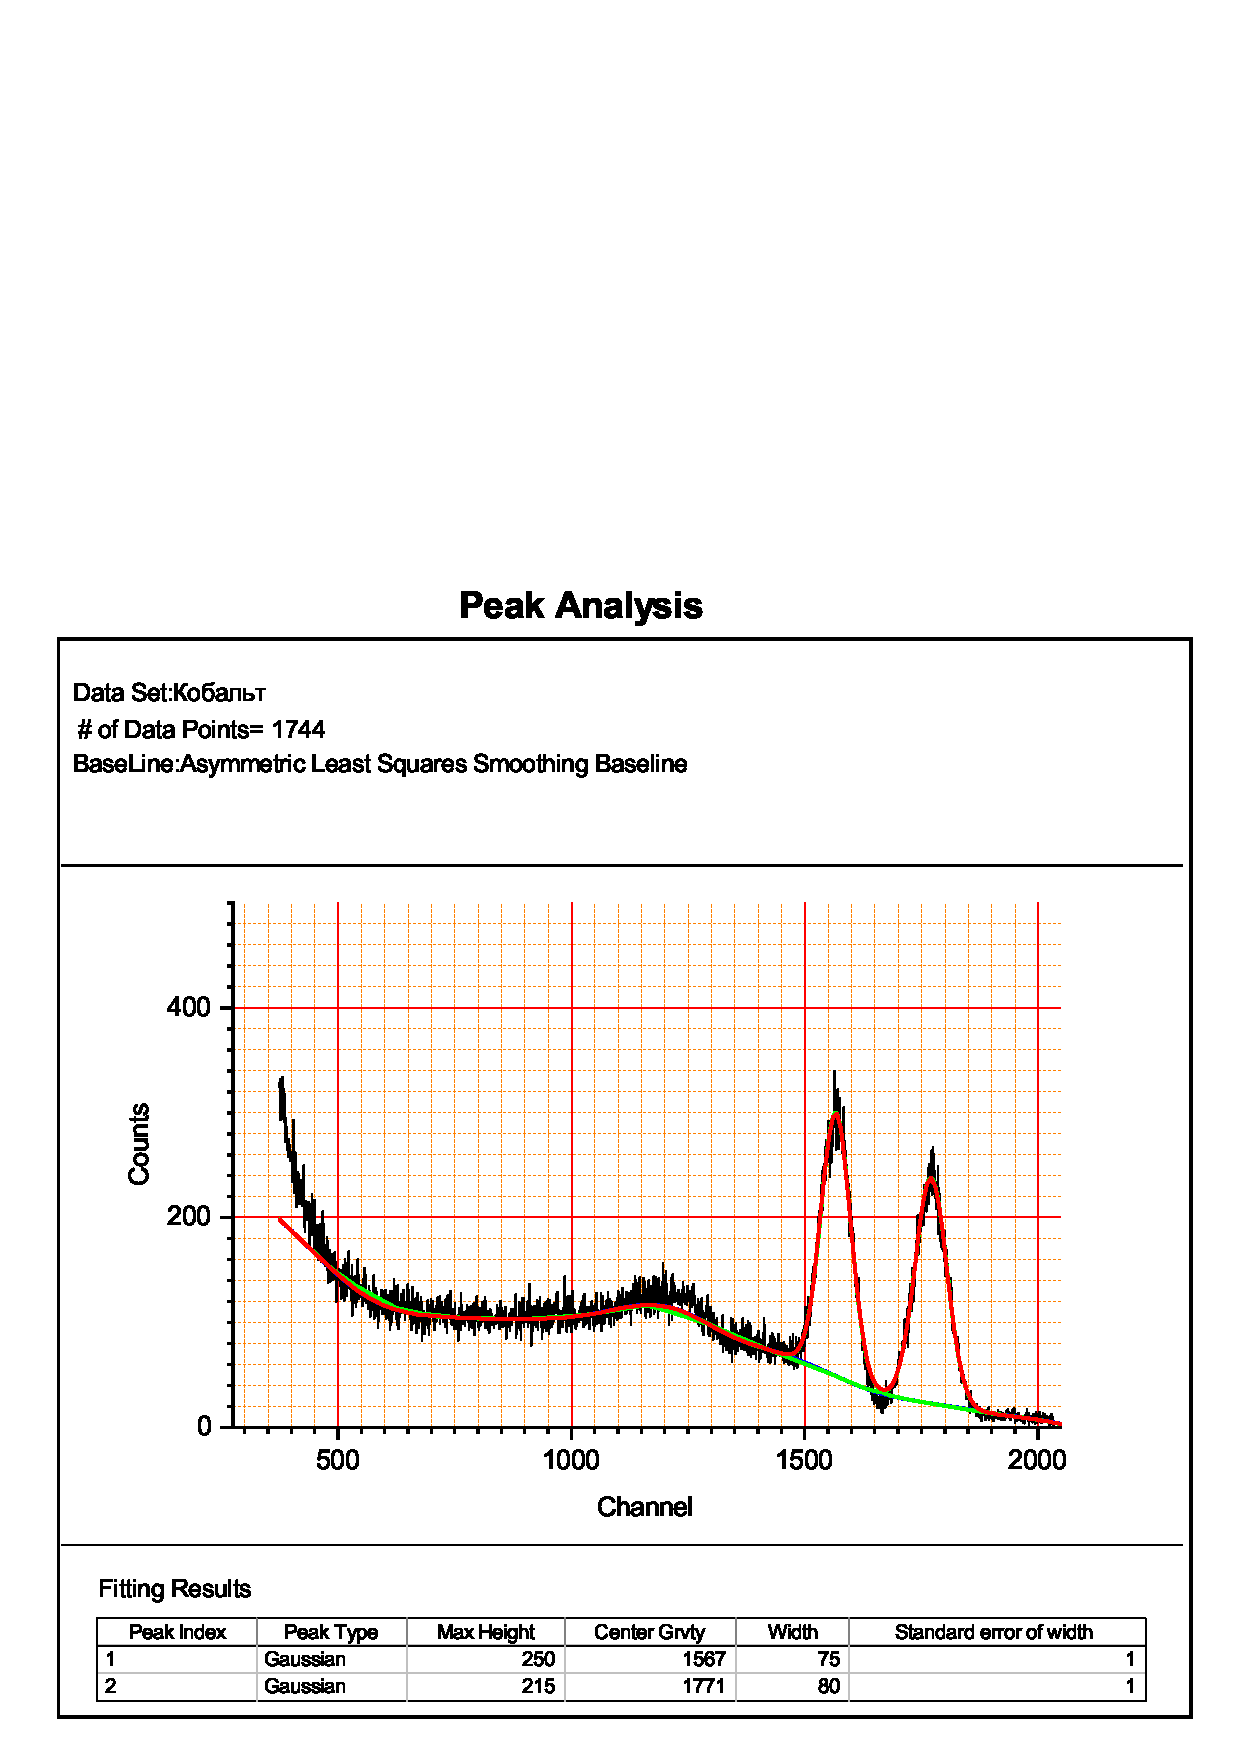
\includegraphics[scale=0.6]{2.jpg}
\end{center}
Как видно из распределния, большинство зарядов расположились в диапазоне $1.3-1.7$. Возьмём их НОД и запишем его как итоговый элементарный заряд:
\begin{center}
\fbox{$e = (1.6 \pm 0.2) \cdot 10^{-19}~\text{Кл}$}
\end{center}
\item Оценим время релаксации, взяв за $t_0$ время частицы с близким к $e$ зарядом -- $t_0 = 10.23~\text{с}$:
\begin{center}
\fbox{$\tau = \dfrac{h}{gt_0} \approx 2\cdot 10^{-6}~\text{с}$}
\end{center}
Также оценим расстояние, которое частица пройдёт за это время:
\begin{center}
\fbox{$s = \dfrac{1}{g}\left(\dfrac{h}{t_0}\right)^2 \approx 4\cdot 10^{-11}~\text{м}$}
\end{center}
\end{enumerate}
\end{document}